\section{Gewichtsfunktion}

In Abbildung \ref{fig:impulse} ist die Gewichtsfunktion $g(t)$, auch Impulsantwort genannt, zu sehen. Diese Funktion ist die Ableitung der Übergangsfunktion $h(t)$, auch Sprungantwort genannt.
\[h(t) \xrightarrow{\frac{d}{dt}} g(t) \]
\[H(s) = \frac{1}{s} * G(s) \xrightarrow{*s} G(s)\]
Die Impulsantwort konvergiert gegen den statischen Verstärkungsfaktor $K=4$: \[lim_{t\to\infty} g(t) = K\]

\begin{figure}[H]
	\centering
	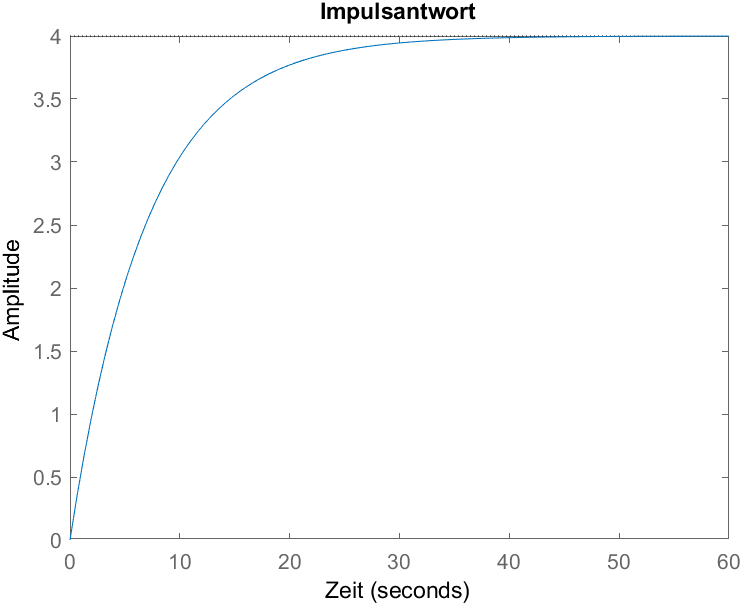
\includegraphics[width=0.8\textwidth]{{diagrams/impulseantwort.png}}
	\caption[Impulsantwort]{Impulsantwort}
	\label{fig:impulse}
\end{figure}